\documentclass[aspectratio=169]{beamer}
\usepackage{CustomTheme}

\addbibresource{Lecture 03.bib}

\title[Intro to CH]{Computational Narrative Analysis}

\begin{document}

%The next statement creates the title page.
\frame{\titlepage}

\section{Introduction}

\begin{frame}{Beyond lexical analysis ?}
    Narrative analysis at scale brings something interesting to literary studies, which is comparison of structures at scale, between centuries, authors, genres and subgenres.

    \vspace{2em}

    We will define in this context ``narrative analysis'' very loosely as any analysis that takes into account succession of events and attempts at defining either the traits of these events or of the succession. 
\end{frame}

\begin{frame}{Today's papers}
    \fullcite{piper2023modeling}

    \vspace{2em}
    \fullcite{operationalizing}
\end{frame}

\section{\textit{Modeling Narrative Revelation}, Piper A. et al., 2023}

\subsection{Question, Context, Definitions}

\begin{frame}{Paper}
    \fullcite{piper2023modeling}
\end{frame}

\begin{frame}{Context \& Main Research Question}
    \begin{itemize}
        \item Stories = Time, which means that Stories = Steps of information dissemination
        \begin{itemize}
            \item ``Independent of what is told, how it is told is a key aspect of a story’s meaning''
            \item ``“discourse structure” [=] an ordering problem, i.e. the discrepancy between how narrative information is revealed and the underlying logic of events within the story''.
        \end{itemize}
        \item Order has been a focus, but not amount and releasing windows.
        \begin{itemize}
            \item ``Given a beginning state of no knowledge about a story and an end state of full knowledge about a story’s contents, what are the rhythms of dissemination through which we arrive at this final state?''
            \item How does this dissemination and its rhythm varies across genres, audiences (youth novels vs adult novels), etc. ? How does it correlates to appreciation \footfullcite{GlobalCoherence} ?  
        \end{itemize}
    \end{itemize}
\end{frame}

\begin{frame}{Three hypothesis}
    \small
    \begin{itemize}
        \item<1-> \textbf{H1. Average Rate of Revelation}. \only<1>{We expect average revelation at the book level to vary by all of our measured social categories. Specifically, prior work [29] has indicated that fictional narratives are more predictable at the sentence level and thus we expect to see lower levels of average revelation with respect to fictionality at the document level. We also \textbf{expect average revelation to be negatively associated with reading level and positively associated with prestige} (more information being more “difficult” for readers to process and thus potentially more valued by elite readerships).}%
        \item<2-> \textbf{H2. The Slope of Revelation}. \only<2>{We expect there to be an \textbf{association between revelation and narrative time}. Prior theoretical work has suggested that narratives exhibit structural patterns [17], which has been confirmed in different ways through empirical work [5, 27, 11]. A general linear increase in surprise would support a theory of narrative investment in the value of plot twists (or “surprise endings”), while a general linear decrease would support the theory of narrative immersion, i.e. once novel information is introduced a narrative spends less time introducing more information (exploration) and more time exploiting known information. \textbf{While we expect there to be an association between revelation and time, prior work does not give clear indications of which directionality to expect}.}%
        \item<3->\textbf{H3. Dependency Patterns of Revelation}. \only<3>{Given assumptions about the value of narrative structure to narrative meaning, \textbf{we expect there to be discernible dependency patterns to the rise and fall of revelation}, with the present extent of revelation driven by that of the past in non-trivial ways (e.g., lagged dependency). While no prior work has suggested that narrative revelation should follow predictable dependency patterns, it could be the case that this is a latent structural feature to narrative plotting and potentially drives reader enjoyment.}
    \end{itemize}
\end{frame}

\subsection{Method}

\begin{frame}{Method and Influences}
    \small
    \begin{itemize}
        \item Methods drawn from information theory and statistics, specifically time series analysis.
        \item Relative Entropy (Kullback-Leibler divergence) to quantify how much new data between $T$ and $T-1$ (non overlapping).
        \begin{itemize}
            \item ``Second, in using an information-theoretic model of narrative revelation, quantifying surprise through similarity of word-count distributions in adjacent windows of text, our models are agnostic with respect to linguistic or thematic content.''
            \item Entropy: ``In thermodynamics, entropy is often associated with the amount of order or disorder in a thermodynamic system.'' (Wikipedia)
            \item Sample 1000 words per 50 equal parts of texts. So texts need to be 50~000 words long minimum.
        \end{itemize}
        \item Time Series Analysis to detect and describe aspects of temporal behaviour.
        \item Dataset is the CONLIT dataset (2700 books, English, 12 genres, contemporary, since 2001)
        \item Focus on 4 metadata: Fiction/Non-Fiction, Prestige, Age Level, Point-of-View (1st/3rd)
    \end{itemize}
\end{frame}

\begin{frame}{Kullback-Leibler divergence}
    \begin{center}
        $D_{KL}(p, q) = \sum_{x \in X} p(x)log(\frac{p(x)}{q(x)})$
    \end{center}\pause %DRAMATIC PAUSE
    
    \begin{itemize}
        \item $X$ (discrete) state space (discontinuous sequence)
        \item $p()$ and $q()$ are probability mass functions defined on $X$, such that $p(x)=0$ implied $q(x)=0$.
        \item $D_{KL}(p, q) \geq 0$
        \item $X_{T}$ is the union of all words in $T$ and $T-1$, where the window is 1000 words.
        \item $x$ is basically a word in $X$ where $X$. $p(x)$ is the relative frequency of $x$ in $T$.
    \end{itemize}
\end{frame}

\begin{frame}{Kullback-Leibler divergence exemplified}
    \centering
    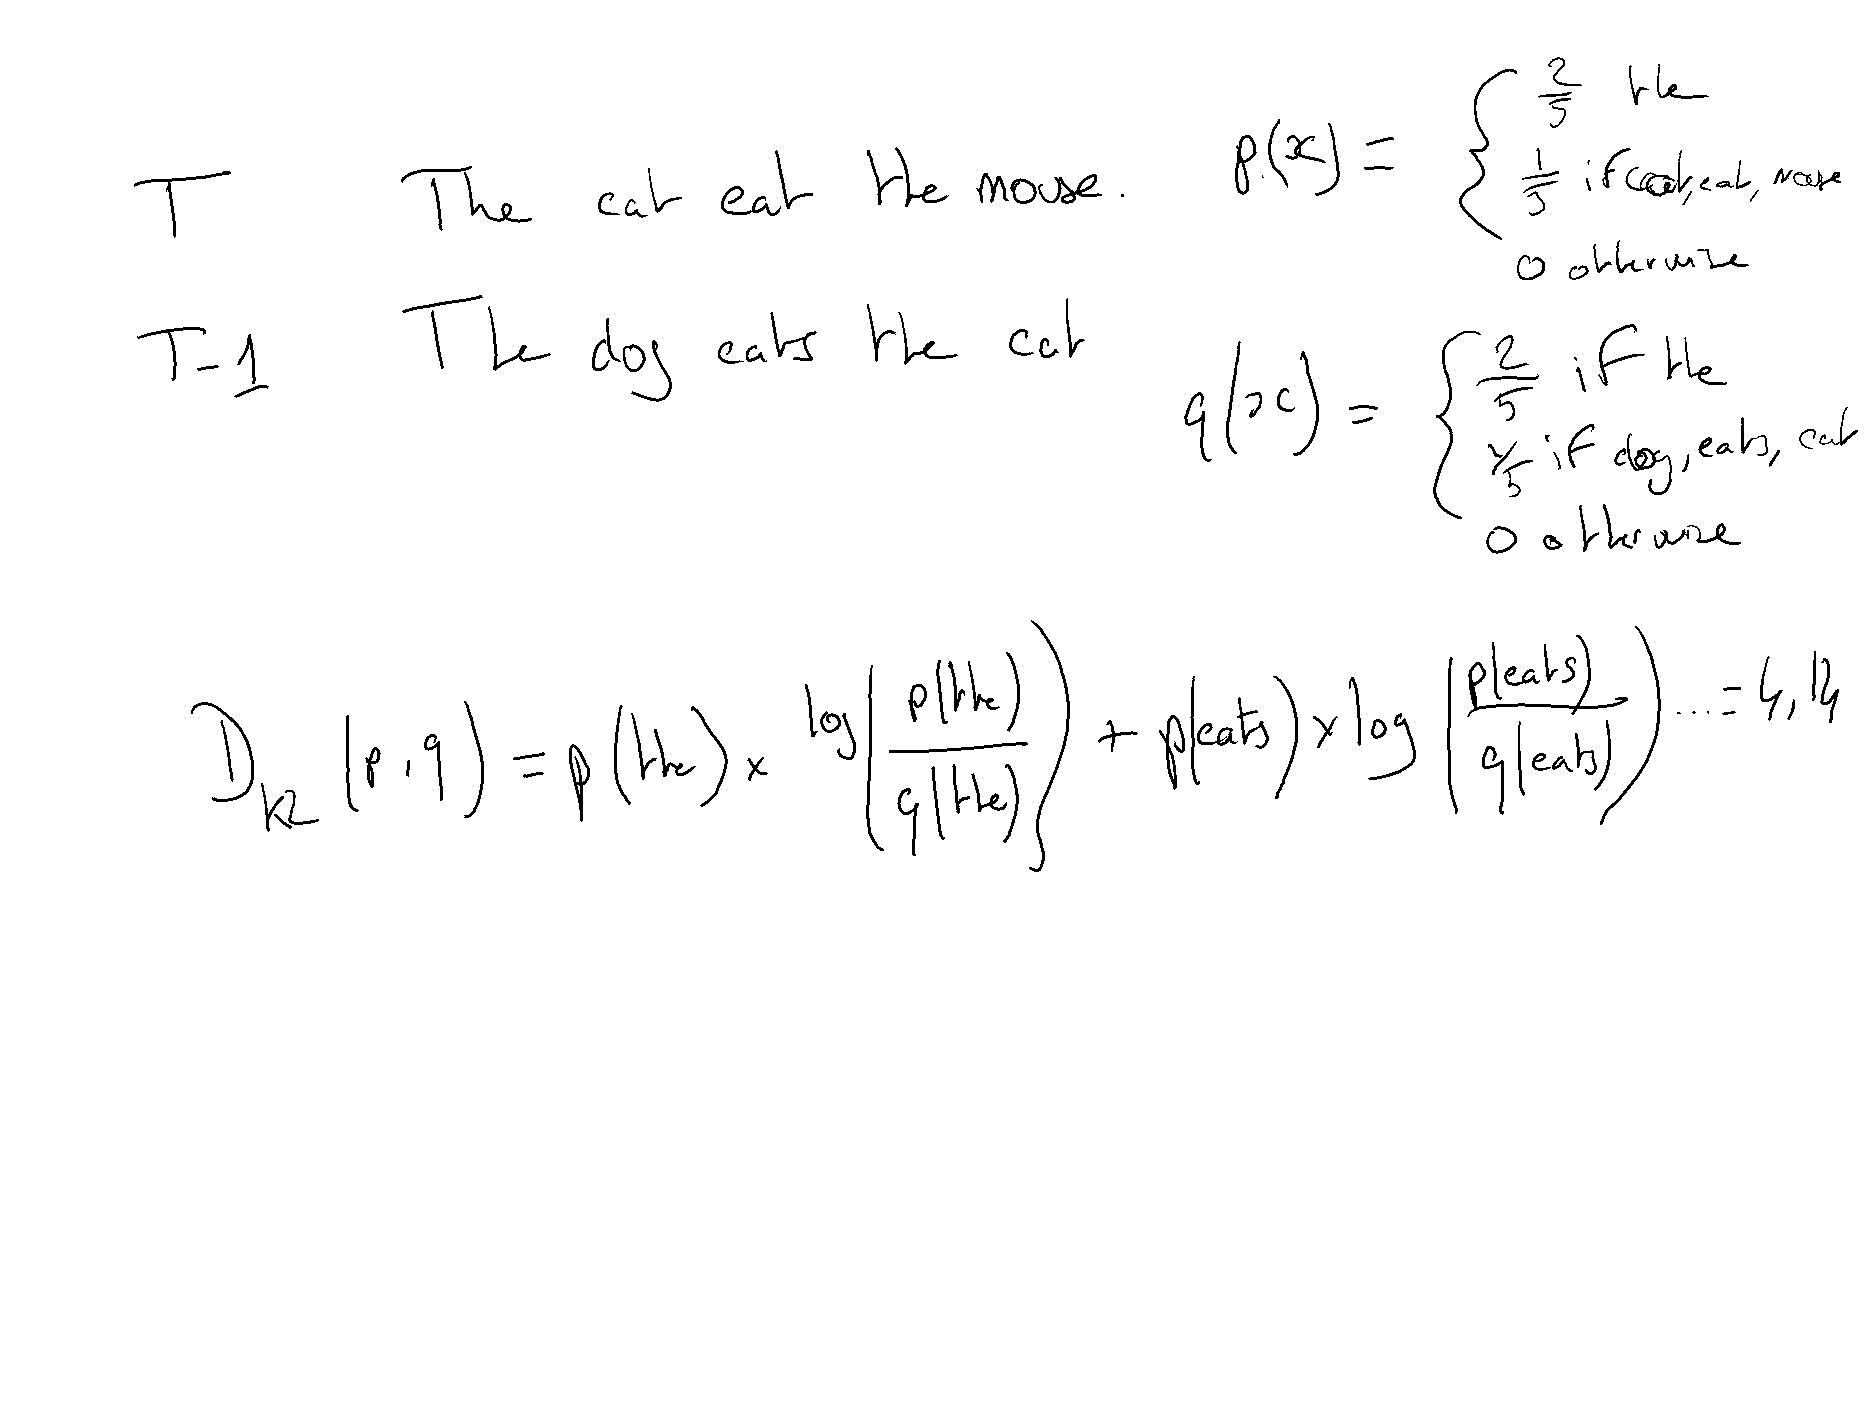
\includegraphics[width=.8\linewidth]{nlp-for-ch/images/dkl.png}
\end{frame}

\begin{frame}[fragile]{Kullback-Leibler divergence applied}

    % \lstset{basicstyle=\tiny,style=myCustomMatlabStyle}
\begin{minted}[fontsize=\tiny]{python}
from collections import Counter
import math

def dkl_funk(sentence_t_minus_1: str, sentence_t: str):
    sentence_t = Counter(sentence_t.lower().split())
    sentence_t_minus_1 = Counter(sentence_t_minus_1.lower().split())
    words = set(sentence_t.keys()).union(sentence_t_minus_1.keys())
    
    def p(w):
        return sentence_t.get(word, 1e-9) / sum(sentence_t.values())
    def q(w):
        return sentence_t_minus_1.get(word, 1e-9) / sum(sentence_t_minus_1.values())
        
    dkl = []    
    for word in words:
        dkl.append(
            p(word) * math.log(p(word) / q(word))
        )
    return sum(dkl)

print(dkl_funk("The cat eats the mouse", "The dog eats the cat"))
>>> 4.144653163244628
print(dkl_funk("The cat eats the mouse", "All of a sudden, a big bear approaches and breaks in"))
>>> 20.06083522879849
\end{minted}
\end{frame}

\begin{frame}{Killback-Leibler Divergence (KBL) applied on 4 texts}
    \centering
    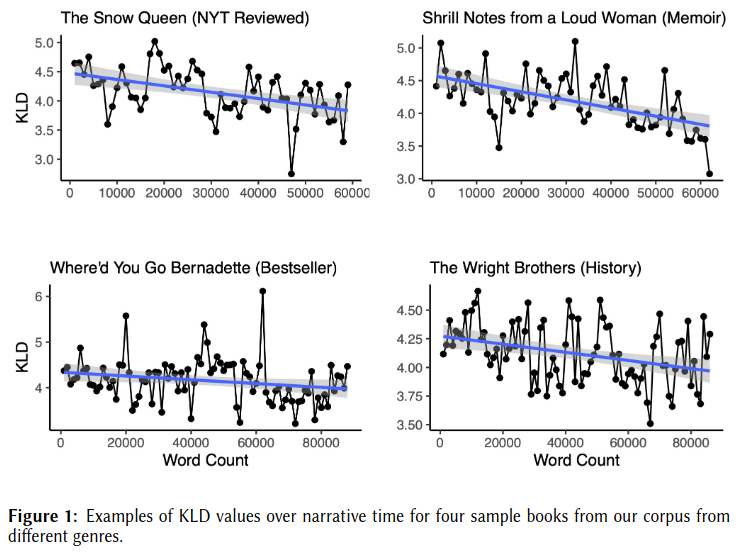
\includegraphics[width=.60\linewidth]{intro-to-ch/images/entrop_examples.png}
\end{frame}

\subsection{Results}

\begin{frame}{Average Revelation Hypothesis (H1)}
    \begin{itemize}
        \item Compute the average value of $KLD_{T}$ over times T, with standardization according to book length in CONLIT data.
        \item Compute Cohen's : $d = \frac{\overline{DKL_{t_{1}}} - \overline{DKL_{t_{2}}}}{\sigma_{T}}$ where $t_{1}$ is one sample and $t_{2}$ another from $T$
        \item \textbf{Results:}
        \begin{itemize}
            \item Non fiction has higher average information revalation over time.
            \item Prestige has the inverse effect, and is twice most impactful as Age Level: contemporaneous prestigious books have lower entropy (lower amount of new information) from one spot to another on average.
        \end{itemize}
    \end{itemize}
\end{frame}

\begin{frame}{The Slope of Revelation (H2)}
    \begin{columns}
        \begin{column}{.7\textwidth}
            
            \begin{itemize}
                \item Regression analysis: find a function that would fit the curve.
                \item Correlates with H1: less and less revelations over time in general
                \item At local minima: the end of books have in general higher KLD (and so new information)
                \item ``We found that youth fiction was similarly associated with greater decreases of revelation over narrative time, but that prestige and point-of-view were not''
            \end{itemize}
        \end{column}
        \begin{column}{.3\textwidth}
            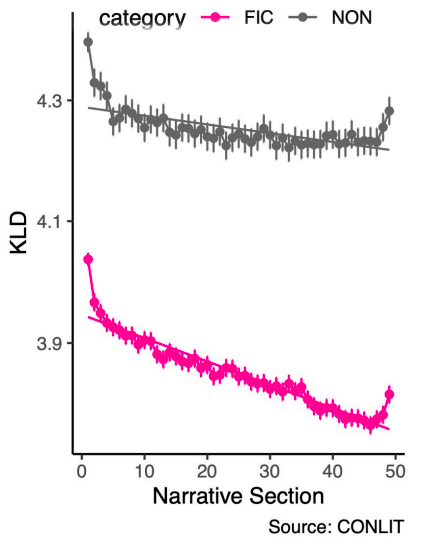
\includegraphics[width=\linewidth]{images/entropy_linear.png}
        \end{column}
    \end{columns}
\end{frame}

\begin{frame}{Dependency Patterns of Revelation (H3)}
    \begin{itemize}
        \item No clear period frequency regarding KLD.
        \item Use of ARIMA models (AutoRegressive, Integrated and Moving Average) who tries to identify the lag $p$ such that $KDL_{T}$ can be predicted by $KDL_{T-p}$ and a trend of order $d$, such that each $KDL_{T_{i}}$ fits a slop of its polynomial order.
        \item For our second variable, 39\% of all books exhibited autoregressive behavior ($d > 0$), meaning that in a strong minority of books the successive values of narrative revelation are correlated.
    \end{itemize}
\end{frame}


\subsection{Discussion}

\begin{frame}{A convincing article}
    \begin{itemize}
        \item The article is sound, well written and builds on previous knowledge, with a strong state-of-the-art \textit{à la} computer science / natural language processing.
        \item It provides not only a new method, but new results. 
        \item Code is not provided, reproducibility is lessened, but the overall explanations should make up for it.
        \begin{itemize}
            \item Overall, no details are given on preprocessing.
        \end{itemize}
        \item The argument against MLM, SLM or LLM is sound: if we don't know what is inside the training data, how can we be sure that the relationship between $T$ and $T-1$ is not skewed by pretraining knowledge ?
    \end{itemize}
\end{frame}

\begin{frame}{With limitations ?}
    \begin{itemize}
        \item The use of word frequencies, as duly noted by the author, and word-to-word comparison lower the impact of the comparison: if I have $X_{T} = \text{I, eat, chocolate}$ and $X_{T-1} = \text{I, buy, kinders}$, is the information revelation that important ? The usage of embeddings to compare words, in one way or another, and map $X$ onto a semantic space with connected frequencies might allow for more fine grained results (see \cite{eder2022boostingwordfrequenciesauthorship}\footfullcite{eder2022boostingwordfrequenciesauthorship}).
        \item A smaller focus, on genres would have been interesting, beyond fictionality.
        \item While the idea of chunking everything the same way and then sampling words makes sense, how does it compare to respecting the author intended structure for the text: chapters, paragraphs ? Would it "clean up" the slope ?
        \item What about turning point detection ? Looking at the original graph, it seems that this might be possible to capture narrative breakpoint...
    \end{itemize}
\end{frame}

\begin{frame}{Questions ?}
    
\end{frame}

\section{\textit{Operationalizing and Measuring Conflict in German Novels}, Haüssler et Gius, 2023}


\begin{frame}{Paper}
    \fullcite{operationalizing}
\end{frame}

\subsection{Question, Context, Definitions}

\begin{frame}{Context \& Main Research Question}
    \begin{itemize}
        \item Conflict is ``considered constitutive for notions of genre'', they are part of the identify of Naturalist texts with their ``societal conflicts''.
        \item Identifying conflict would enable their classification and then their evaluation as (non-)defining traits of genre, periods, authors, etc.
        \item So can we identify conflict is the main question, but the question arises specifically at the sentence level.
    \end{itemize}
\end{frame}

\begin{frame}{(Re-)Defining Conflict}
    Conflict is defined as an incompatibility by the authors between two agents
    \begin{itemize}
        \item where one of the agent experiences or imagines ``an incompatibility in perceiving, thinking, feeling and wanting with the other agent'';
        \item Incompatibility can then be defined as factual or hypothetical, it does not need to be true to be experienced.
        \item Incompatibility can be of values, as the negative appreciation of one's acts or thoughts, such as mocking one's actions: they define it as the negative appreciation of an experience.
        \item Incompatibility can root itself in the divergence of experience: ``I am a worker, you are the company's boss daughter, we are from different worlds.'' is an incompatibility, and a such should be a conflict ?
    \end{itemize}
\end{frame}

\begin{frame}{Defining Conflict around Axes}
    \begin{columns}
        \begin{column}{.5\linewidth}
            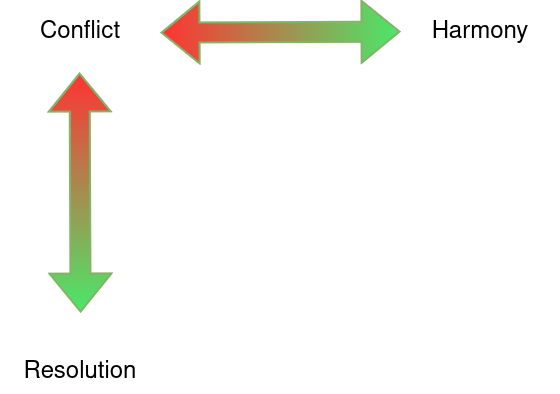
\includegraphics[width=\linewidth]{intro-to-ch/images/ConflictDetection.drawio.png}
        \end{column}
        \begin{column}{.5\linewidth}
            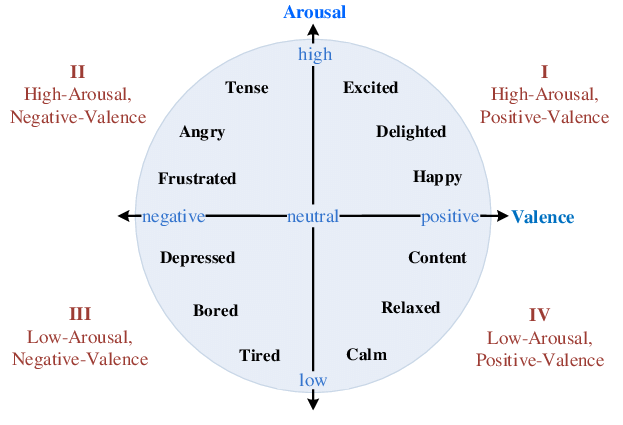
\includegraphics[width=\linewidth]{intro-to-ch/images/Two-dimensional-valence-arousal-space.png}
        \end{column}
    \end{columns}
    \vspace{1em}
    {\footnotesize Image from the right taken from \fullcite{buildingaffectiveresources}}
\end{frame}

\subsection{Method}

\begin{frame}{Method}
    \begin{itemize}
        \item Manual annotation and evaluation of the definition through the evaluation of inter-annotator agreement.
        \begin{itemize}
            \item IAA setup a bit skewed, with an author (professor) and a student participating.
        \end{itemize}
        \item Overall, 107 sentences out of 1000 random sentences showed incompatibility with some form of agreement between both annotators, but that represents a mere 44\% of kept sentences between both annotators. Of these, only a few display hypothetical incompatibility (the number of kept sentences is unclear between actual and hypothetical). Cohen's Kappa = .325 (Low)
        \item Cohen's Kaappa is a function of probabilities: $\frac{P(Agreement) - P(Random)}{1 - P(Random)}$. 
        \begin{itemize}
            \item $P(Agreement)$ is the frequency of agreement between two annotators
            \item $P(Random)$ is the sum of the product of frequencies per class acros annotators such that $P(Random) = P(\text{Inc}, \text{Annotr}_{1}) * P(\text{Inc}, \text{Annotr}_{2}) + P(\text{NotInc}, \text{Annotr}_{1}) * P(\text{NotInc}, \text{Annotr}_{2})$
        \end{itemize}
    \end{itemize}    
\end{frame}


\begin{frame}{Computational approach}
    \begin{itemize}
        \item Train Word Embeddings following a previous paper using Gensim.
        \item Preprocessing: lemmatization, punctuation removal, lowercased text.
        \item Compute the value of a word $w$ in a sentence $W$ \ref{formula:value_w}, where $L$ is the set of positive and negative labels across Arousal, Valence, Conflict vs. Harmony, Conflict vs. Resolution. Then value of a sentence $W$ is the average of value(w) (see \ref{formula:value_W}).
    \end{itemize}
    \begin{equation}
        \text{value}(w) = \frac{%
            \sum_{l \in L_{neg}}%
            cos(\overrightarrow{w}, \overrightarrow{l})}{\overline{L_{neg}}} - \frac{%
            \sum_{l \in L_{pos}}%
            cos(\overrightarrow{w}, \overrightarrow{l})}{\overline{L_{pos}}}
        \label{formula:value_w}
    \end{equation}
    \begin{equation}
        value(W) = \frac{\sum_{w \in W}value(w)}{\overline{W}}
        \label{formula:value_W}
    \end{equation}
\end{frame}

\subsection{Results}

\begin{frame}{Comparison of results}
    \begin{itemize}
        \item Huge disagreement between manual and automatic annotation, with an important set of false positive (high precision, TP/ TP + FP) and an overall low recall (TP / TP + FN).
        \item Only one situation where the recall is higher than 50 \%, but this leads to an abysmal precision (11\% of matches are correct)
    \end{itemize}
\end{frame}

\begin{frame}{Analysis of automatic annotation}
    \centering
    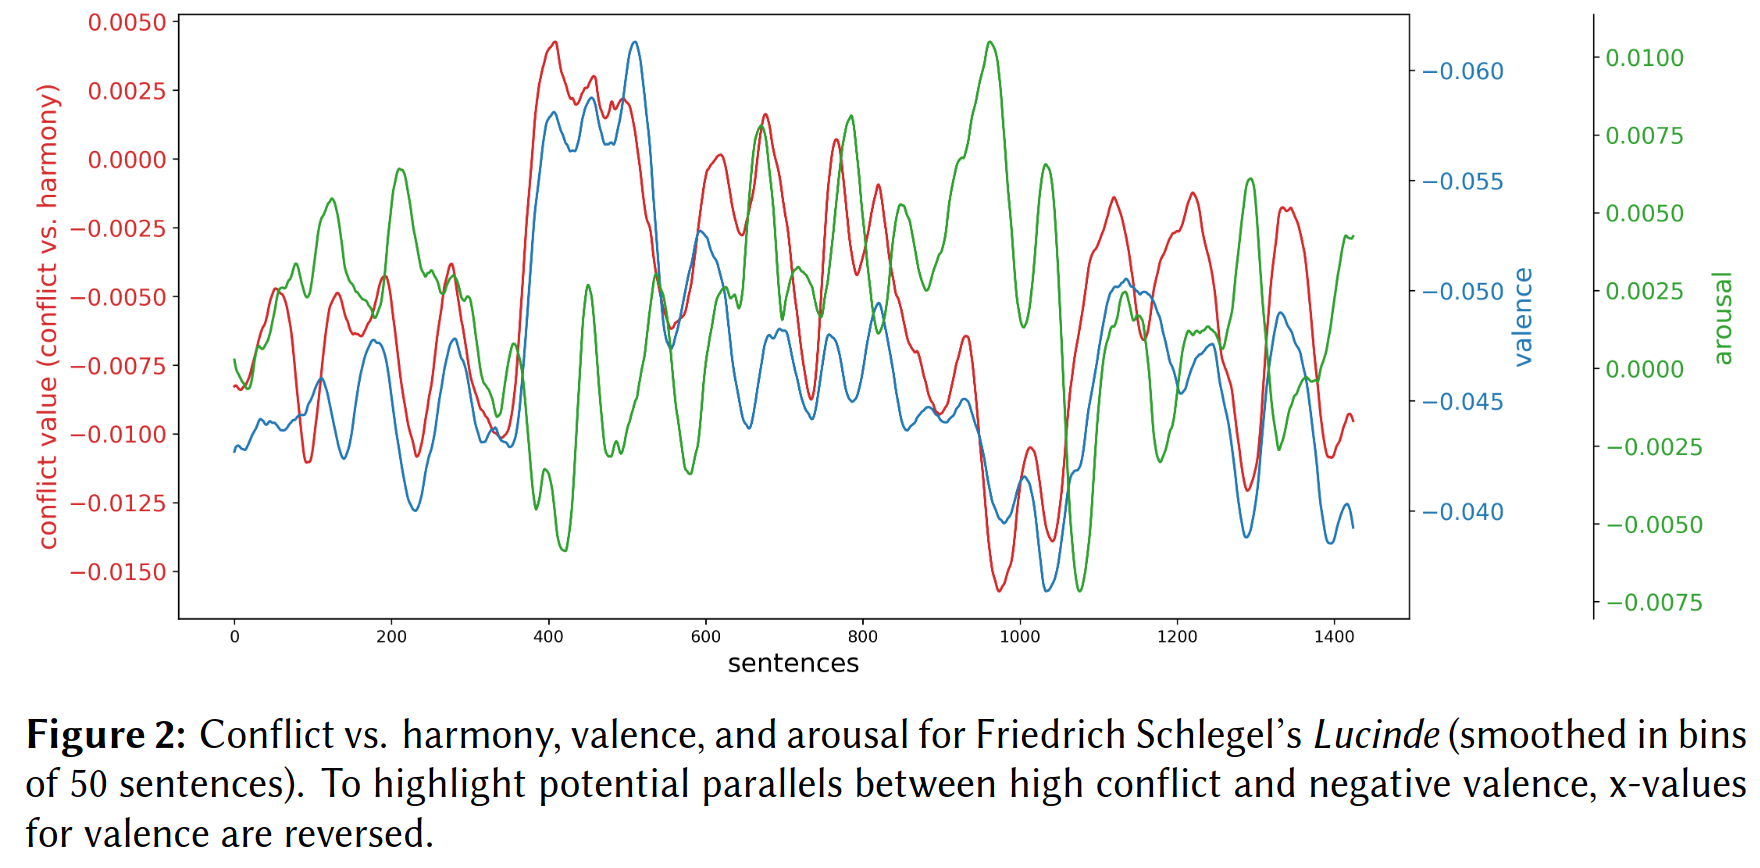
\includegraphics[width=.9\linewidth]{intro-to-ch/images/plotarousal.png}
\end{frame}

\begin{frame}{Conclusion of the paper}
    \begin{itemize}
        \item Definition needs refining for operationalization;
        \item Word embeddings needs to be further analyzed.
    \end{itemize}
\end{frame}

\subsection{Discussion}

\begin{frame}{Computational approaches as restriction ?}
    \begin{itemize}
        \item The definition of conflict purely at the sentence level is a first problematic point. It requires the text to be concise yet express incompability around an object -- that needs to be described --  between two agents who need to be identified.
        \item This issue of the sentence-level definition of conflict is clearly shown when the authors, to showcase one example of hypothetical incompability, provide a three-replica dialog page 428:
        \begin{itemize}
            \item  “»No, my father is and will remain your and your husband’s faithful friend.« »Well,« said Mrs. Ebermann, »I would feel a cessation of his interest in us painfully, but a reproach would not arise from it in my heart.«” (Ida Boy - Ed: (1892) Empor, [Authors] translation). 
            \item Would this approach work with both sentence taken independently ? Is the first sentence ``Conflict resolution'' because of \textit{remain} and the second one hypothetical conflict because of \textit{feel}, \textit{cessation}, \textit{interest}, \textit{reproach}, \textit{would} ?
            \item By lemmatizing, how much of the hypothetical is lost through the normalization of would to will ? Or here probably \textit{würde} $\rightarrow$ \textsc{werden}
        \end{itemize}
    \end{itemize}
\end{frame}

\begin{frame}{An issue with the redaction and some of the method}
    \only<1,3>{
    \begin{itemize}
        \item The way things are written makes it harder to follow the  argument: in the paper, the comparison of automatic annotation through embeddings and manual annotation comes AFTER the automatic application of the embeddings. How can the reader appreciate the value of the automatic annotation with having any kind of metrics regarding its effectiveness before hand ?
        \item The results are treated using a binary threshold around 0 or quartiles. It would have been interesting to finetune the threshold according to k-Fold experiments, where we split all positive and negative matches in 5 batches, decide on a threshold value where 4 batches have the best true positive rate and false negative ratio, and then evaluate on the last batch. 
        \item<3> Because what we capture is conflict, and that this is a binary situation, we need to make sure things are filtered.
    \end{itemize}
    }
    \only<2>{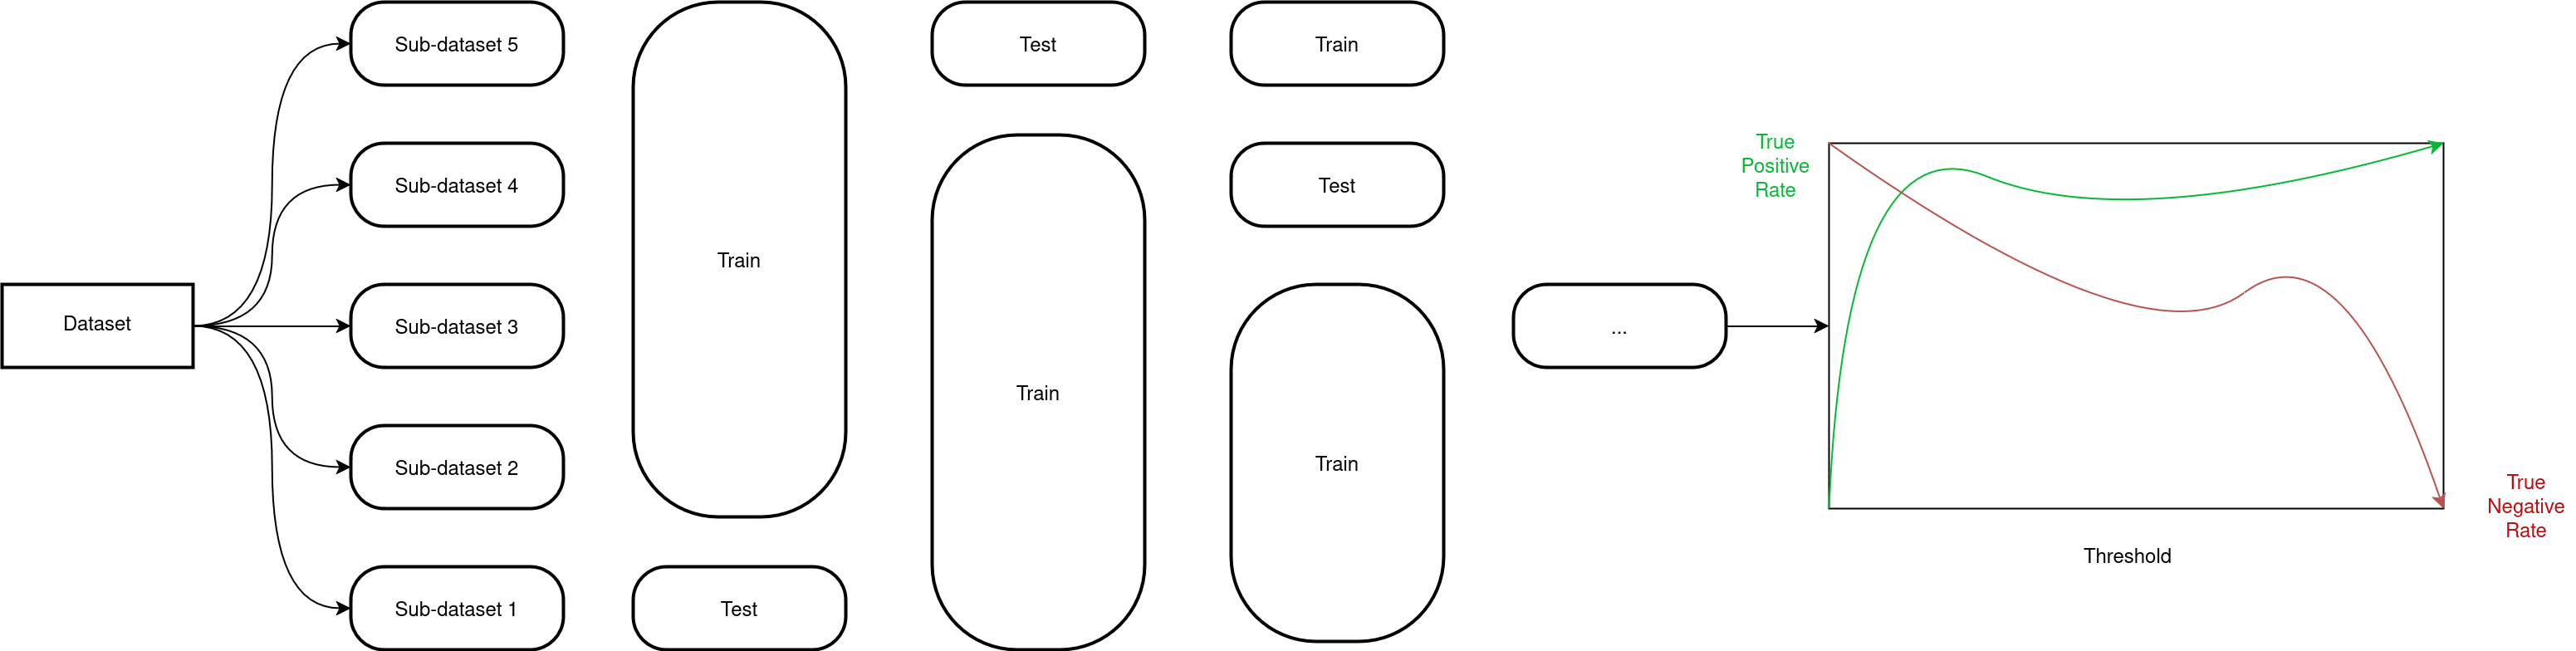
\includegraphics[width=\linewidth]{intro-to-ch/images/PrecisionCurve.drawio.png}}
\end{frame}

\begin{frame}{The issue of a word-based approach ?}
    \only<1,3>{
        \begin{itemize}
            \item The presence of words, and their proximity with labels, does not say anything about the syntactical construction. While semantic of single words may approximate conflict, sentence such as ``I am a worker, you are the company's boss daughter, we are from two worlds.'' does not include a single lexical clue about conflict, but builds conflict through the opposition of words and the implied limits it produces...
            \item There was actually no analysis of the proximity of the label words, which results in an ``unknown space of disagreement''.
            \item<3> The lack of fine-tuning on the proximities, the filtering of words, or even 
        \end{itemize}
    }
    \only<2>{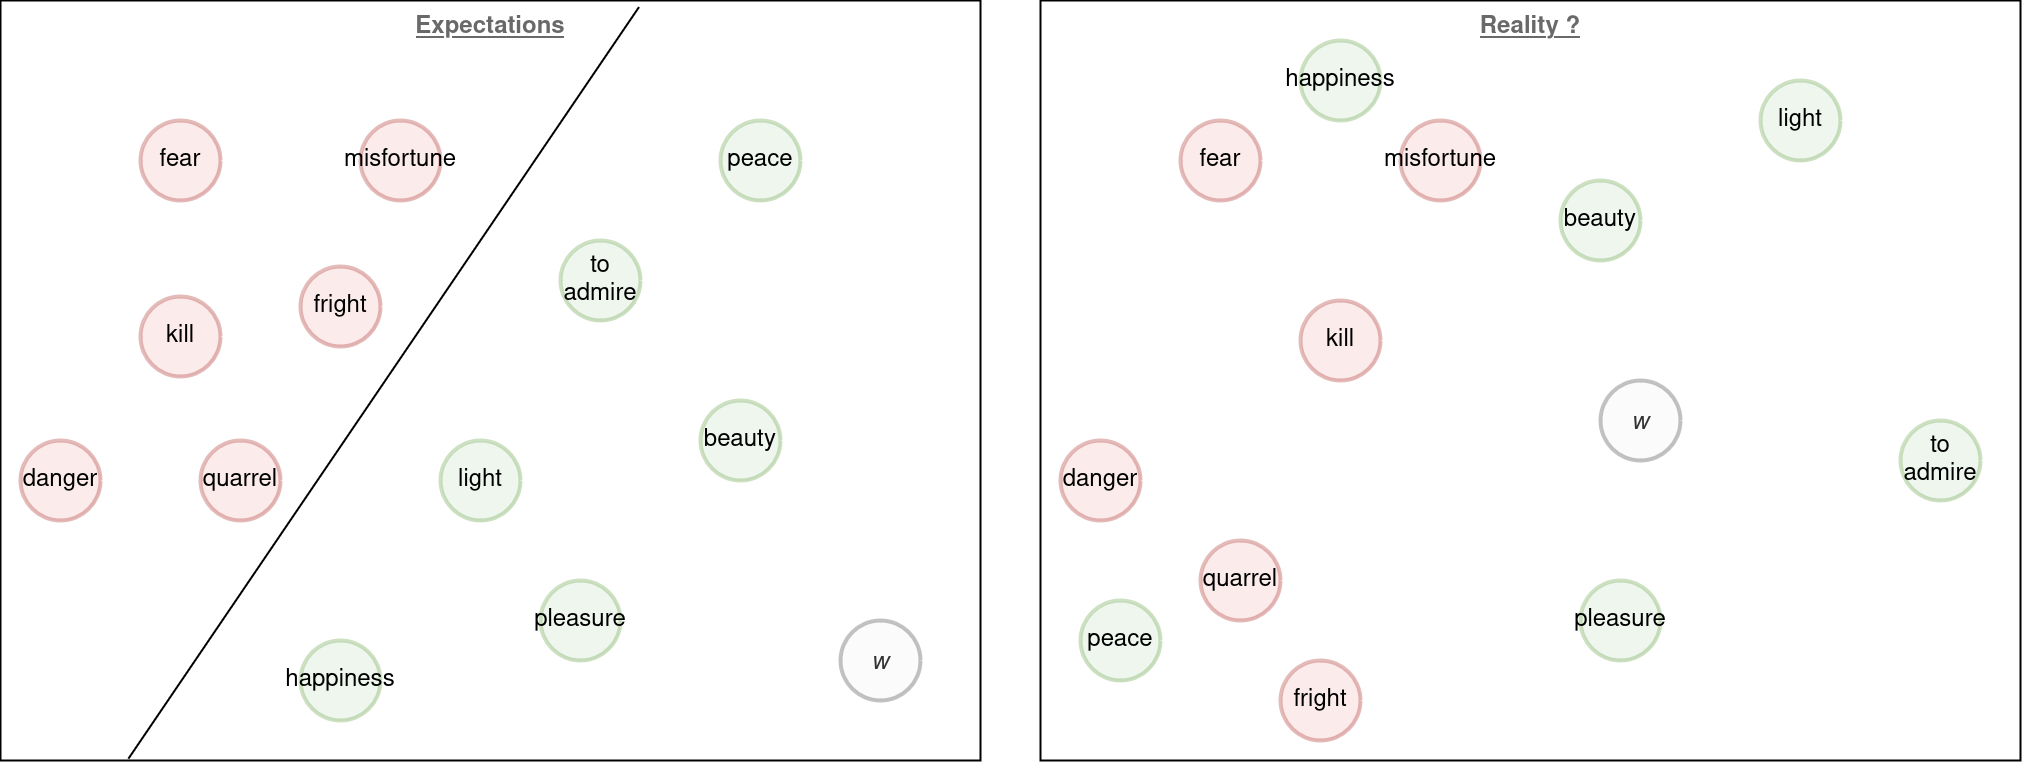
\includegraphics[width=\linewidth]{intro-to-ch/images/Spaces.drawio.png}}
\end{frame}

\begin{frame}{An alternative approach ?}
    \begin{itemize}
        \item Ok, if even trying to figure out thresholds that yields better results, which means spaces are quite well separated, does not work, what can we do ?
        \item Keeping word approach, maybe keeping even the original forms but using a modern embedding, and training a model to fit the decision made by the human annotators, as a sentence classification problem.
        \item Leaving the word2vec embedding, still at the sentence level, using Bert sentence encoding and then classifying ?
        \item Few shot learning using Large Language Model, which have shown capacity for reasoning ?
        \item Using previous and next sentence as contextual information vectors ?
    \end{itemize}
\end{frame}

\begin{frame}{Questions ?}
    
\end{frame}

\section{Next week}

\begin{frame}{Next week}
    Mike Kestemont and Ecological Models applied to Cultural Heritage Loss Estimations !    
\end{frame}

\end{document}